\documentclass[17pt]{extarticle}
\usepackage{../mystyle}

\begin{document}
\section{Алгоритм симплекс-метода, симплекс-таблицы}
\begin{enumerate}
    \item Для известного начального базиса находят координаты разложения векторов \( b \) и \( A_k \) \( (k = 1, \ldots, n) \) по базису:
          \[
              \begin{cases}
                  x^0 = A_B^{-1}b - \text{ненулевые координаты опорной точки}, \\
                  x^k = A_B^{-1}A_k, \, k = \overline{1,n} - \text{координаты разложения вектора } A_k \text{ по базису}.
              \end{cases}
          \]
    \item Вычисляют симплекс-разности: \(\Delta_k = c_k - c_B A_B^{-1}A_k, \, k = 1, \ldots, n. \)
    \item Проверяют план на оптимальность. Если все \(\Delta_k \leq 0\), \( k = 1, \ldots, n \), то решение оптимально.
    \item Проверяется критерий отсутствия решения.
          Если \(\exists \Delta_r > 0\): все \( x_{ir} \leq 0, i = \overline{1,m} \), то целевая функция не ограничена сверху в допустимой области.
    \item Определяют вектор \( A_r \), вводимый в базис: \(\Delta_r > 0\)
          и максимальная среди всех положительных \(\Delta_k\), \( k = \overline{1,n} \).

    \item Определяют вектор \( A_s \), выводимый из базиса:
          \[
              A_s : \frac{x_{s0}}{x_{sr}} = \min_{i \in I} \frac{x_{i0}}{x_{ir}} \quad (x_{ir} > 0) \Rightarrow \text{строим новый базис и переходим в п.1.}
          \]
\end{enumerate}
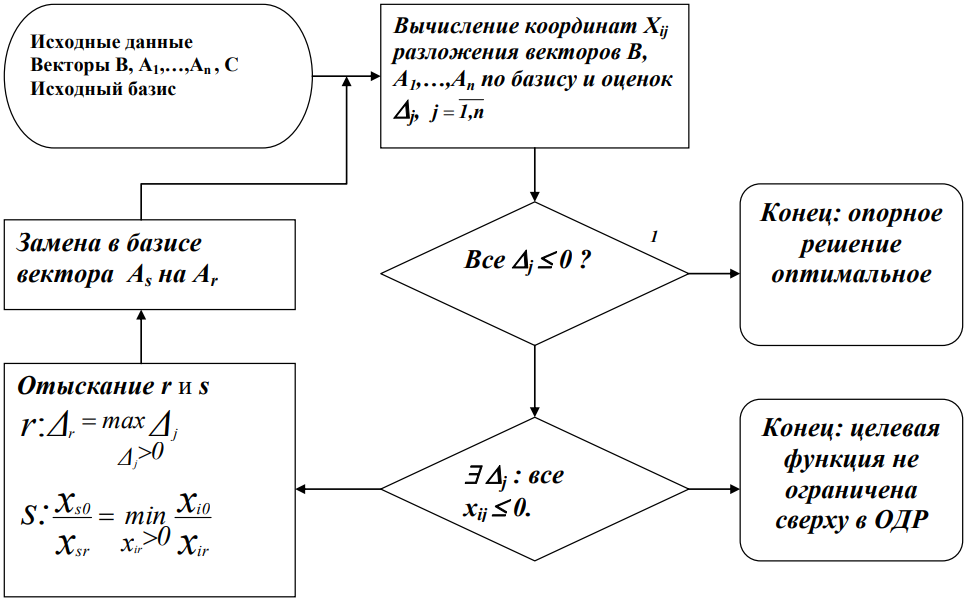
\includegraphics[width=1\textwidth]{9.png}
Формулы пересчета координат разложения векторов по новому базису:

\[
    x_{jk}' =
    \begin{cases}
        x_{jk} - \frac{x_{jr}}{x_{sr}} x_{sk}, & \text{если } j \in I \setminus s, \\
        \frac{x_{sk}}{x_{sr}},                 & \text{если } j = r.
    \end{cases}
\]

\begin{tabular}{|c|c|c|c|c|c|c|c|}
    \hline
                 &                      &                         & \( C_1 \)      & \(\cdots\) & \( C_r \)      & \(\cdots\) & \( C_n \)      \\
    \hline
    базис        & \( C_{\text{баз}} \) & \( B \)                 & \( A_1 \)      &            & \( A_r \)      &            & \( A_n \)      \\
    \hline
    \( A_{i1} \) & \( C_{i1} \)         & \( X_{10} \)            & \( X_{11} \)   &            & \( X_{1r} \)   &            & \( X_{1n} \)   \\
    \hline
    \(\vdots\)   & \(\vdots\)           & \(\vdots\)              & \(\vdots\)     &            & \(\vdots\)     &            & \(\vdots\)     \\
    \hline
    \( A_{is} \) & \( C_{is} \)         & \( X_{s0} \)            & \( X_{s1} \)   &            & \( X_{sr} \)   &            & \( X_{sn} \)   \\
    \hline
    \(\vdots\)   & \(\vdots\)           & \(\vdots\)              & \(\vdots\)     &            & \(\vdots\)     &            & \(\vdots\)     \\
    \hline
    \( A_{im} \) & \( C_{im} \)         & \( X_{m0} \)            & \( X_{mr} \)   &            & \( X_{mr} \)   &            & \( X_{mn} \)   \\
    \hline
                 &                      & \( f(x^{\text{опт}}) \) & \( \Delta_1 \) &            & \( \Delta_r \) &            & \( \Delta_n \) \\
    \hline
\end{tabular}
\end{document}